\section{Evaluation Report Targets Table}
\label{sec:eval_report_targets}

Every Evaluation report obtains a special section 'Targets', where all unique targets 
are listed which could be evaluated for the selected standard and data sources. \\

It is important to note that, although this table only contains the target information relevant to the specific Evaluation result stored in the report,
it represents the same targets listed in the 'Targets' tool of the Flight Deck. 
Thus, in case the targets stored in the database are modified (e.g. by recomputing the unique targets, modifying the Evaluation usage and constraints via the 'Targets' tool, etc.), 
the Evaluation results will need to be refreshed in order to again bring them up-to-date with the database targets. \\

The table can be used both for documentation purposes and easy modification of target Evaluation usage and 
constraints directly from the Evaluation report. \\

The 'Targets' section can be selected from the table of contents using the 'Sections' button.

\begin{figure}[H]
  \hspace*{-2cm}
  \center
    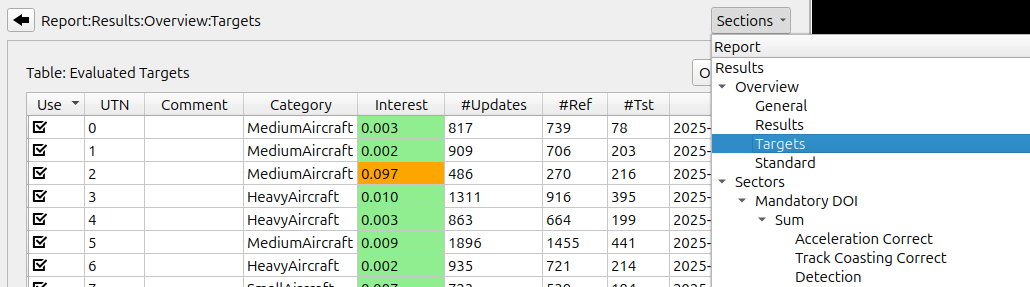
\includegraphics[width=15cm,frame]{figures/eval_targets_section.png}
  \caption{Show Evaluation targets table}
\end{figure}

The section then presents itself as follows.

\begin{figure}[H]
  \hspace*{-2cm}
  \center
    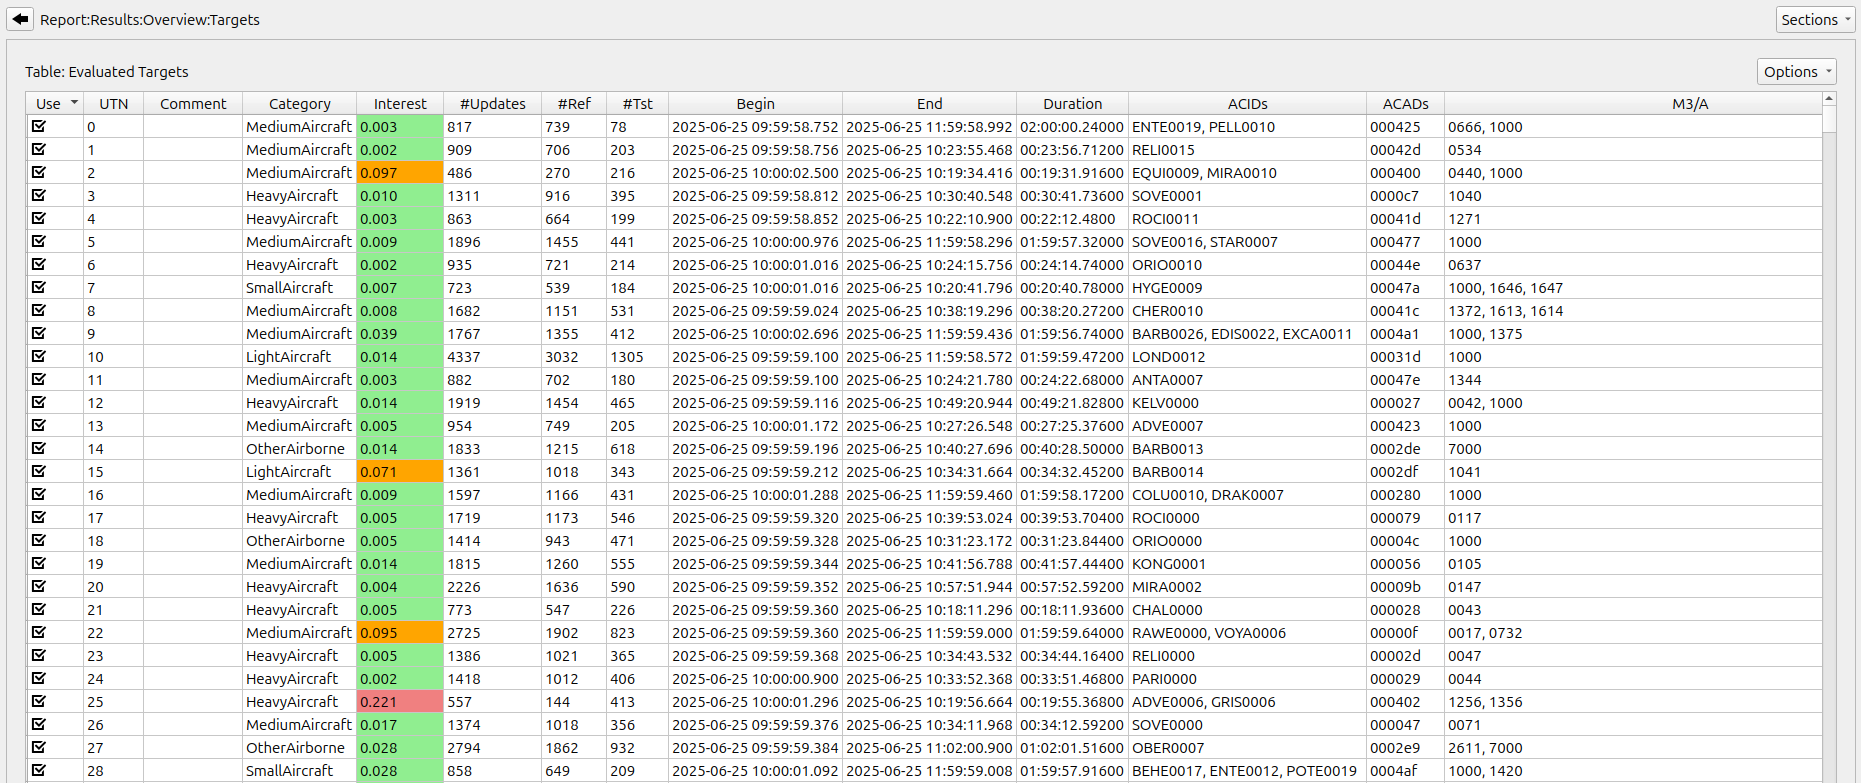
\includegraphics[width=17cm,frame]{figures/eval_targets_table.png}
  \caption{Evaluation targets table}
\end{figure}

The following columns exist:

\begin{itemize}  
  \item Use: Icon indicating Evaluation usage and constraints, as specified in section \nameref{sec:ui_eval_usage}
  \item UTN: Unique Target Number
  \item Comment: User comment, as specified in the 'Targets' tool of the Flight Deck
  \item Category: The target's emitter category
  \item Interest: Score showing how strong a negative impact a target had on all requirement results. Please refer to \nameref{sec:eval_targets_of_interest} for details.
  \item \#Updates: Sum number of target reports
  \item \#Ref: Number of target reports in reference data
  \item \#Tst: Number of target reports in test data
  \item Begin: First timestamp of UTN
  \item End: Last timestamp of UTN
  \item Duration: Duration in HH:MM:SS.SSS
  \item ACIDs: Mode S aircraft identification(s)
  \item ACADs: Mode S aircraft address (hexadecimal)
  \item M3/A: Mode 3/A code(s) (octal)
\end{itemize}
\ \\

Unless otherwise specified, the column content reflects the values from both reference and test data. \\

\subsection{Targets of Interest}
\label{sec:eval_targets_of_interest}

\begin{figure}[H]
  \hspace*{-2cm}
    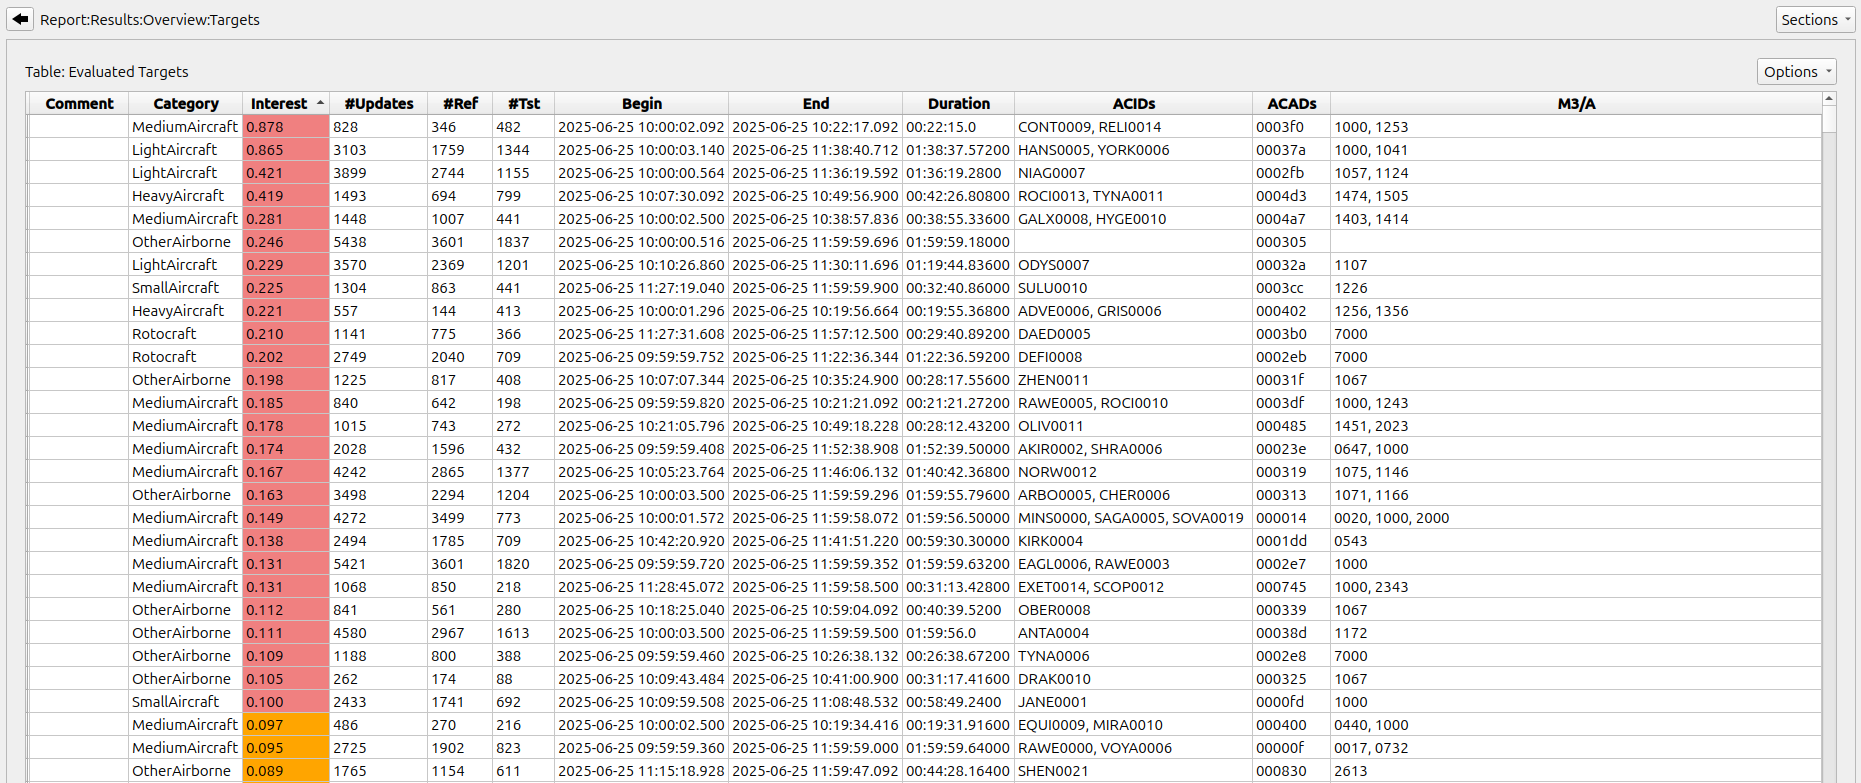
\includegraphics[width=18cm,frame]{figures/eval_targets_interest.png}
  \caption{Evaluation targets with evaluated data sorted by interest}
\end{figure}

After running an evaluation, in the Evaluation Targets tab, the displayed interest is a numerical score showing how strong a negative impact a target had on all requirement results. \\

The interest factor is calculated by:
\begin{itemize}  
\item Stepping through all targets in all given sectors and requirements
\item For each target and requirement, the negative contribution of said target to the respective requirement is calculated
\begin{itemize}  
\item Resulting in a value between 0 (no negative impact) and 1 (all negative contributions come from this single target)
\end{itemize}
\item For each target an accumulated sum of per-requirement interest factors is calculated
\end{itemize}
\ \\

The coloring is performed as follows:
\begin{itemize}  
\item higher than 0.1: red
\item higher than 0.05 and lower than 0.1: orange
\item 0.05 and below: green
\end{itemize}
\ \\

When right-clicking a target, several options are shown:

\begin{itemize}  
\item Show full UTN: Load all data from the respective target (not just used reference / test data)
\item Show Surrounding Data: Load all data surrounding the target in position and time (e.g. to find association issues)
\item Jump to requirement: Jump to the respective requirement results section
\item Target Usage: Set a target's Evaluation usage and constraints, as described in section \nameref{sec:eval_targets_of_interest_usage}
\end{itemize}
\ \\

When using the 'Options' button and selecting the submenu 'Edit Shown Interest Factors', a list of all requirements is displayed to select which interest values should be aggregated.

\begin{figure}[H]
  \hspace*{-2.5cm}
    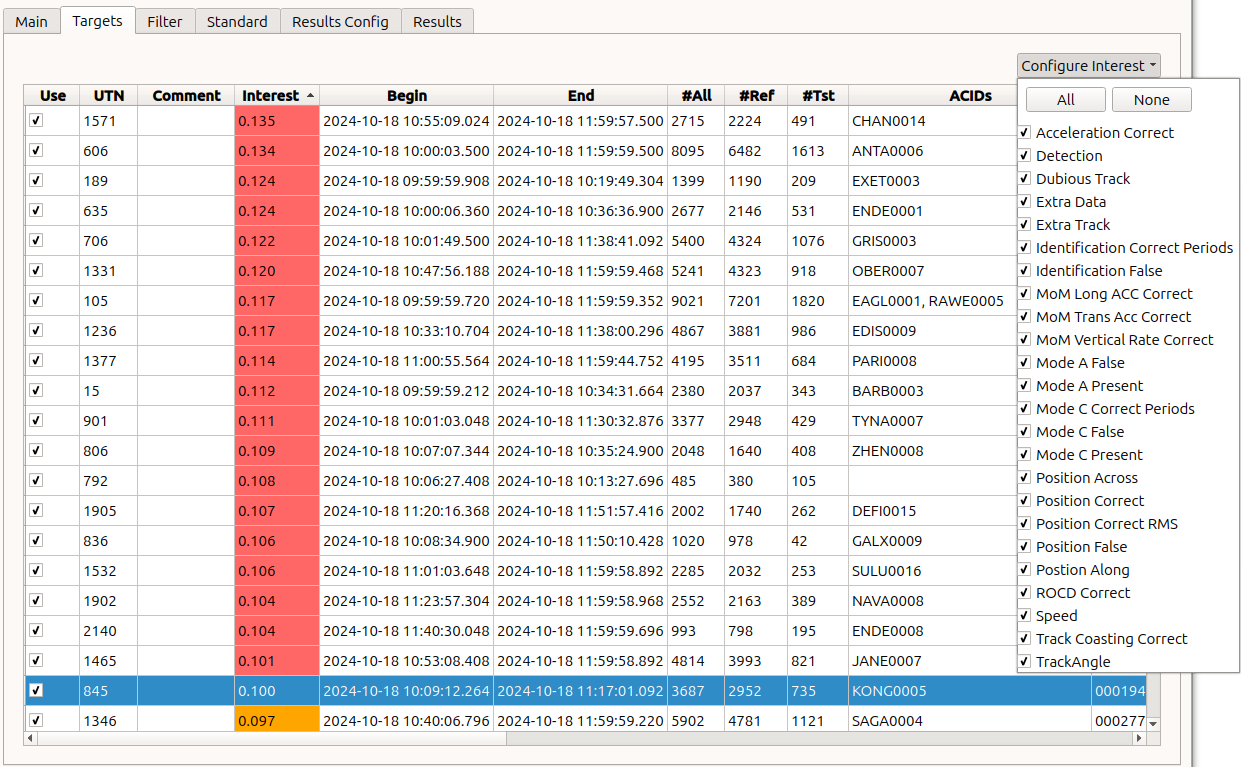
\includegraphics[width=19cm,frame]{figures/eval_targets_config_interest.png}
  \caption{Evaluation targets: Configure interest}
\end{figure}

\subsection{Editing Evaluation Target Usage and Constraints}
\label{sec:eval_targets_of_interest_usage}

Using the Evaluation report's 'Targets' table, a target's Evaluation usage and constraints 
can be directly edited right from the Evaluation report, instead of having to switch to the 
list of unique targets shown in the 'Targets' tool of the Flight Deck. \\

Right-clicking on a target and selecting 'Target Usage' will show the following menu.

\begin{figure}[H]
  \hspace*{-2cm}
  \center
    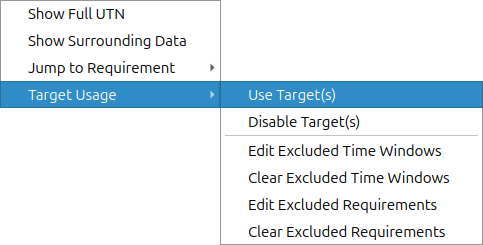
\includegraphics[width=10cm,frame]{figures/eval_target_usage.png}
\end{figure}

The specified actions are the same as described in section \nameref{sec:ui_eval_usage}.
Please refer to this section for more details about each action. \\

Triggering these actions will modify the targets stored in the database,
and this will set Evaluation reports to out-of-date state, as their listed results are no longer up-to-date. \\

Pressing an Evaluation report's 'Refresh' button will update the report accordingly,
and the new result can be inspected. This way, after a closer inspection, certain targets can be removed from Evaluation, 
removed from certain requirements, removed for certain time windows and so on.
The report will adapt to these changes after a refresh.

